% !Mode:: "TeX:UTF-8"
% 文字编码:UTF-8
\chapter{相关研究工作}
\label{chap:related}

\section{实时视频传输码率自适应算法}
自互联网诞生以来,数据传输过程中的拥塞控制就一直是研究的重点。传统拥塞控制方法,如TCP,通过拥塞窗口 \cite{jacobson1988congestion} 控制数据传输过程,拥塞窗口的大小决定了当前能发送的数据数量。为了探测网络带宽,拥塞窗口缓慢增加,一旦检测到网络拥塞,则大幅度降低窗口大小,以求迅速恢复。研究 \cite{wu2000end}指出,大部分基于拥塞窗口的控制算法都包含了数据包的重传,因此不适用于对延迟敏感的实时数据传输。为了适应实时数据传输的需要,研究 \cite{turletti1996videoconferencing} 提出了一种基于码率调整的拥塞控制方法,这一方法直接估计当前网络带宽并以此设置数据发送速率。结合视频编码码率可变的特性,这一基于码率的拥塞控制方法也成为实时视频码率自适应算法的基础。

尽管TCP由于重传机制无法被实时视频传输采用,但其对网络带宽上限进行探测的思路却在视频码率自适应算法中得到了继承。一种经典思路就是以网络丢包率作为拥塞信号对码率进行调整,如研究\cite{wu2000end}中采用算法
\begin{algorithmic}
\If {$(P_{loss} \le P_{threshold})$}
    \State $r := min\{(r+AIR), MaxRate \} $
\Else
    \State $r := max\{(\alpha * r), MinRate \} $
\EndIf
\end{algorithmic}
其中$P_{loss}$为当前丢包率,$P_{threshold}$为判断网络拥塞的丢包率阈值,$r$是发送数据的码率,$AIR$为每次码率增加的数值。容易看出这是一种“加性增,乘性减”(Additive Increase Multiplicative Decrease, AIMD)的策略。与之相应的是 研究 \cite{turletti1996videoconferencing} 中提出的“乘性增,乘性减”(Multiplicative Increase Multiplicative Decrease, MIMD)策略。

一种更加直接的拥塞控制方式是通过对网络建模,显式地预测网络带宽的数值。如研究 \cite{floyd1999promoting} 中给出的码率估算模型
\begin{equation}
  r \le \frac{1.5\sqrt{2/3} * MTU}{RTT * \sqrt{p}}
\end{equation}
其中$MTU$(Maximum transit unit)为当前网络最大传输单元,$RTT$(Round Trip Time)为数据包往返时延。与此类似的还有专为多媒体流传输设计的TFRC(TCP Friendly Rate Control) 协议 \cite{handley2003tcp},该协议能够合理控制码率上升速度以避免引起网络上其他TCP数据流的``饥饿''现象。注意到很多基于模型的拥塞控制算法已经引入了传输延迟作为网络探测的信号,如TCP Vegas \cite{brakmo1995tcp} 、TCP-LP \cite{kuzmanovic2003tcp}、LEDBAT \cite{shalunov2012low}等,这有利于实时传输中对延迟的控制。然而上述大部分算法主要利用延迟作为避免与TCP过度竞争的手段,实际应用中仍然存在延迟累积等问题。

\begin{figure}[htbp]
  \centering
  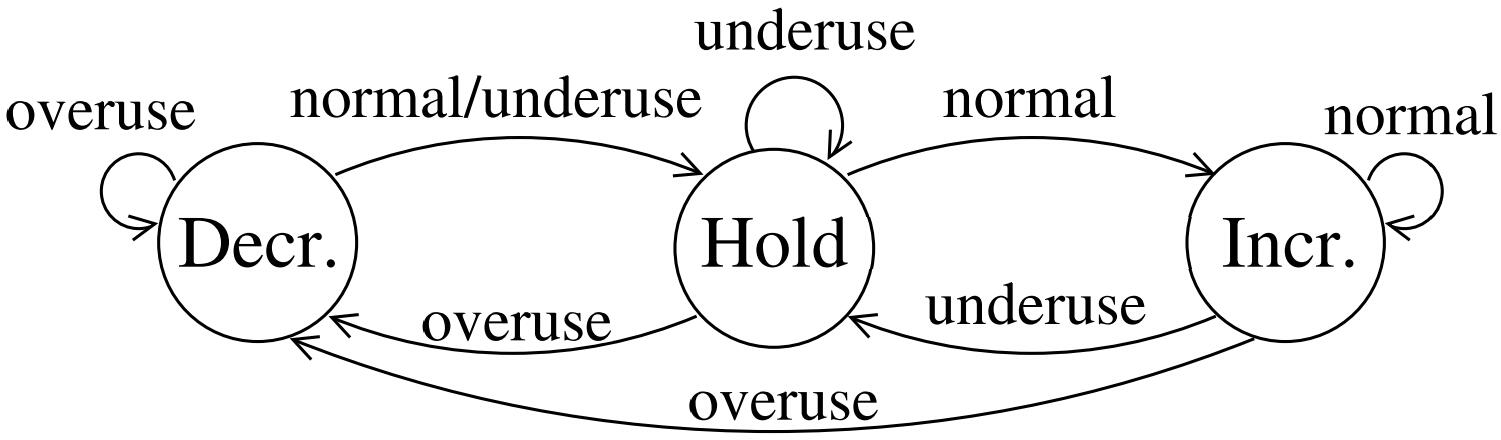
\includegraphics[width=0.7\textwidth]{gcc_state.jpg}
  \caption{WebRTC算法的有限状态机模型}
  \label{fig:gcc_state}
\end{figure}

以上用于实时视频的码率自适应方法都在很大程度上借鉴了传统拥塞控制算法的思想,而随着近年来互联网的发展,实时视频服务的研究在学术和工业界都获得了大量的关注。随着Skype、FaceTime、WebRTC等视频通话应用的兴起,一系列全新的码率自适应算法也随之出现。研究 \cite{de2013experimental} 分析了Google在WebRTC中采用的发送、接收端混合码率自适应算法。其发送端采用基于丢包率的MIMD算法,并综合了TFRC算法
\begin{equation}
  r_t = \left\{ \begin{array}{ll}
    max\{X_t, r_{t-1}(1-0.5p)\} &   p > 0.1\\
    1.05(r_{t-1} + 1kbps)       &   p < 0.02\\
    r_{t-1}                     &   otherwise
  \end{array} \right.
\end{equation}
其中$X_t$为TFRC算法模型估算出的网络带宽。接收端采用了基于网络延迟的算法,并用图 \ref{fig:gcc_state} 所示的有限状态机描述延迟变化趋势,状态间跳转通过专门的网络探测逻辑实现。其相应码率计算公式为
\begin{equation}
  r_t = \left\{ \begin{array}{ll}
    \eta r_{t-1} &   Increase\\
    \alpha R_t   &   Decrease\\
    r_{t-1}      &   Hold
  \end{array} \right.
\end{equation}
其中$R_t$为接收端统计的当前接收速率。在开源VoIP软件Linphone \cite{website:linphone}的底层代码中,也发现了使用有限状态机对网络状态进行检测并针对不同状态应用不同码率调整策略的算法。

尽管实时多媒体流传输的码率控制问题已经获得了大量关注并在学术和工业界出现了各种算法,但目前还没有一种算法在效果方面得到广泛认同。目前互联网工程任务组(The Internet Engineering Task Force, IETF)仍有一个工作组RMCAT \cite{website:rmcat} 负责收集用于音视频实时传输的拥塞控制算法。这也是在我们的研究中努力解决的一个问题。


\section{实时视频流的非对称差错保护}
\label{section:fec_intro}
在网络传输过程中,由于网络拥塞、路由器转发错误、信道错误等问题不可避免地会发生丢包。视频编码传输过程中为了压缩数据量采用的帧内和帧间压缩策略使其对数据错误十分敏感,一旦发生错误或丢包,可能对视频解码过程产生非常严重的影响,造成连续多帧的失真 \cite{stockhammer2003h}。因此我们有必要在传输过程中进行差错控制。

信道上的差错控制技术就是传统的信道编码,是为了克服信道错误而采取的必要措施。信道编码在发送端以某种确定的关联规则(约束)计算校验码元或监督码元,附在被传输的信息序列上。接收端按照既定的规则检查相应码元,如果传输过程中有信息错误或丢失,将会检测到关联信息的变化,从而实现发现错误,乃至纠正错误 \cite{陈敏2004网络实时视频传输研究} \cite{wang1998error} \cite{wang2000error} 。
基于信道编码的差错控制主要包括检错重传和前向纠错两种:
\begin{description}
    \item[检错重传(Auto Repeated Request, ARQ) \cite{soltani2009delay}\cite{schier2012optimizing}] 通过在发送数据包中添加一定冗余编码达到检错目的。接收端进行完整性检验,一旦发现丢包,则向发送端反馈重传请求,发送端重新发送数据包。此过程一直重复直到接收端收到正确的数据包。这是TCP协议中最重要的数据保障策略,然而在实时传输中并不适用。
    \item[前向纠错(Forward Error Correction, FEC) \cite{nafaa2008forward}] 通过向发送数据中添加一定量冗余数据,同时提供数据检错和纠错能力。只要错误和丢包数量不超过一定阈值,接收端就可以解码恢复所有原始数据。这一方法不需要反馈信道,比TCP实时性好 \cite{davis1996joint},因此是需要纠错能力的实时视频传输中常用的方法。
\end{description}

\begin{figure}[htbp]
  \centering
  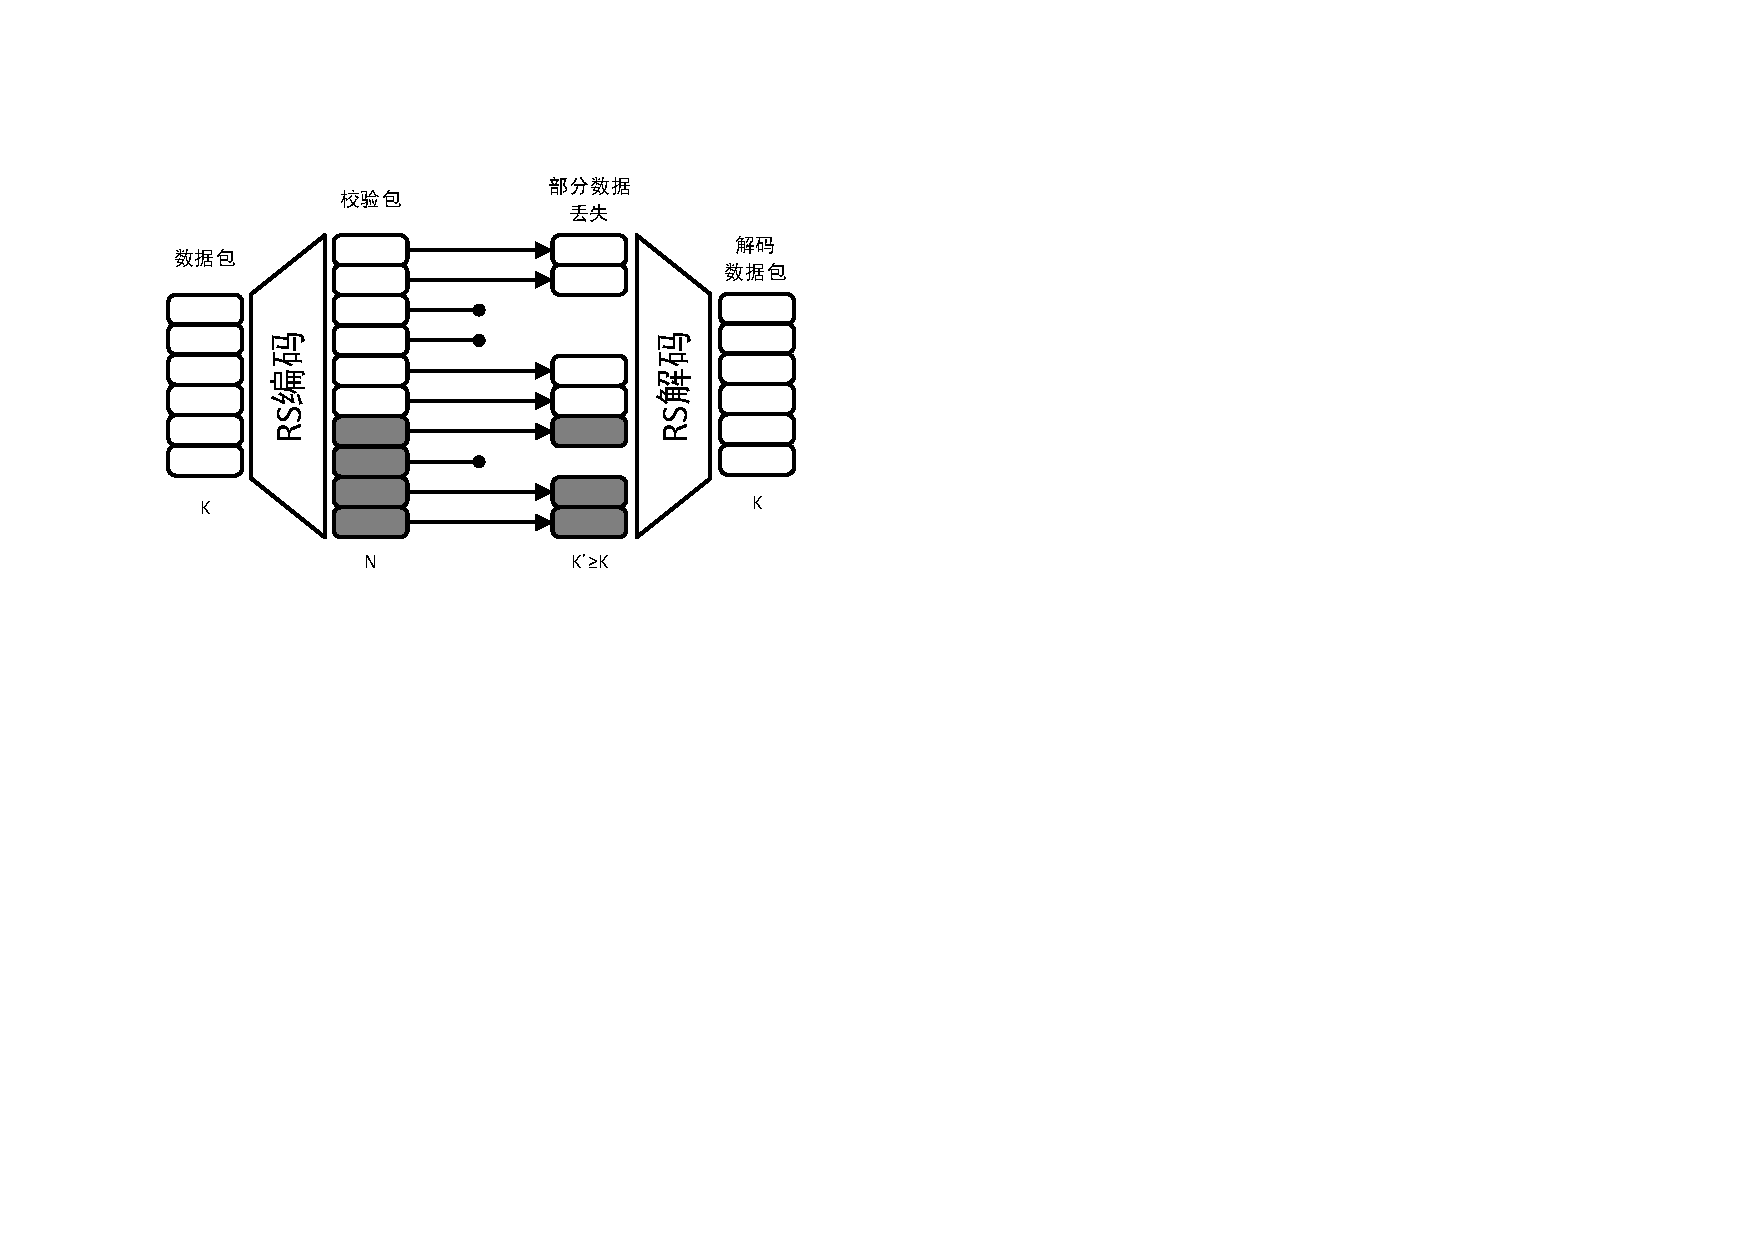
\includegraphics[width=0.7\textwidth]{RS_n_k.pdf}
  \caption{Reed-Solomon码}
  \label{fig:RS_n_k}
\end{figure}

在实时流媒体传输中,使用最多的FEC编码包括LDPC \cite{richardson2003error}和Reed Solomon(RS)编码 \cite{wicker1999reed},它们也是在RTP协议中推荐的差错保护编码方式。RS 编码是一种扩展的非二进制BCH码,在$GF(2^m)$域上进行运算。典型的RS码可以用$RS(N,K)$表示,其中$N$为编码码块长度,$K$为码块中的信息长度,$k=N-K=2t$表示校验码的符号数,$t$表示能纠正的错误数目。另外如果错误位置已知,那么RS码可以纠正$k$个错误。RS码也是一种系统码,即$K$ 个信息码元在编码之后不会发生改变。RS码的简要编解码过程如图\ref{fig:RS_n_k}所示。

在实时视频数据流中,不同位置的数据重要性是不同的。例如在MPEG中,I 帧具有比 P 帧更重要的地位,而P帧又比B帧重要。研究 \cite{yang2005unequal} \cite{zhang2011transmission} \cite{zhang2012novel} \cite{zhou2014novel}表明,在视频传输中使用非对称的冗余编码能够获得更好的差错保护效果。研究 \cite{yang2005unequal} 中提出基于失真权重的预期错误传播长度优化模型进行冗余分配。研究 \cite{zhang2011transmission} 利用失真最优化的思路对冗余分配问题进行抽象表示如下:
\begin{equation}
\begin{aligned}
& \underset{\vec F}{\min}D(\vec F) =
& &  \sum_{j=1}^J D_j P_R(N_j, K_j) \\
& \text{s.t.}
& & R_C(\vec F) \le R_T - R_S \\
\end{aligned}
\end{equation}
其中$D_j$表示第$j$个BOP(Block of Pictures)的整体失真,$P_R$是$RS(N_j, K_j)$进行冗余编码后的丢包率,$R_C(\vec F)$表示冗余分配的码率限制。求解这一带约束的优化问题即可得到最优冗余分配。然而,大部分FEC 框架的冗余保护效果依赖于较大的编码块,而包含多帧数据的编码块会引入额外的播放延迟,这对实时视频传输的效果有很大影响\cite{wang2000error}。

\begin{figure}[htbp]
  \centering
  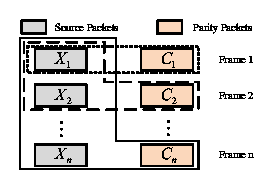
\includegraphics[width=0.6\textwidth]{ew-fec.eps}
  \caption{扩展窗口FEC编码框架}
  \label{fig:ew_fec}
\end{figure}

随着相关研究的深入,一种能解决FEC编码块大小和额外延迟之间矛盾的扩展窗口RS编码框架(Expanding Window Reed-Solomon code, EW-RS)被提出 \cite{sejdinovic2009expanding}。 该框架编码过程如图\ref{fig:ew_fec} 所示,GOP 中第$n$个视频帧的冗余数据包$C_n$包含的编码块由第$1\le i\le n$ 帧的所有数据包组成。通过这一扩展窗口的编码块设置,编码块大小在不引入额外播放延迟的条件下得到了很大的增加。值得一提的是,这一框架还包含了非对称差错保护思想,即越靠前的数据包得到越多的保护。在\cite{sejdinovic2009expanding} 和 \cite{nazir2011expanding} 中,基于扩展窗口的喷泉编码模型被提出;基于扩展窗口的可伸缩视频编码(SVC)也在\cite{vukobratovic2009scalable} 和 \cite{hellge2011layer} 中被提出。在一项最近的工作\cite{xiao2013real} 中,作者提出了基于源数据包随机交换的Reed-Solomon 扩展窗口编码框架。
